% =====================================================================
% figE  — R/ggplot2 -> tikzDevice (parallel to ../figures-tex/figE_deletion.tex)
% Canonical-JSON-only. Regenerate: Rscript figures/make_figures_ieee.R
% Provenance (JSON path :: field = plotted value), one line per series:
% SOURCE: results/C3_u1_blockB_L8_seeds_u5.json :: aggregate.within_probe_mean_across_seeds = 0.4610
% SOURCE: results/U1_E1_transplant_GATE_L12_s{0,1,2}.json :: mean(keycos.within_probe_mean) = 0.6626
% SOURCE: results/C3_u1_blockB_L14_seeds_u5.json :: aggregate.within_probe_mean_across_seeds = 0.5191
% SOURCE: results/G1_L12_analysis.json :: aggregate.within_probe_mean_across_seeds (rewrite ref) = 0.6018
% SOURCE: results/u1_gate_refusal_L12_s0.json :: arms['known=True|edit_ok=False'].nondc_rho = 0.6571
% SOURCE: results/u1_gate_refusal_L12_s0.json :: arms['known=True|edit_ok=False'].dc_rho = 0.4371
% SOURCE: results/u1_gate_eos_L12_s0.json :: arms['known=True|edit_ok=False'].nondc_rho = 0.6530
% SOURCE: results/u1_gate_eos_L12_s0.json :: arms['known=True|edit_ok=False'].dc_rho = 0.4823
% SOURCE: results/u1_gate_suppress_L12_s0.json :: arms['known=True|edit_ok=False'].nondc_rho = 0.6213
% SOURCE: results/u1_gate_suppress_L12_s0.json :: arms['known=True|edit_ok=False'].dc_rho = 0.1587
% SOURCE: results/U1_E1_transplant_GATE_L12_s{0,1,2}.json :: mean(mean_signed_damage) = 3.7888
% SOURCE: results/U1_E1_transplant_GATE_L12_s{0,1,2}.json :: mean(SxC_within_probe_mean) = 0.6779
% SOURCE: results/U1_E1_transplant_GATE_alphadelete_L12_s{0,1,2}.json :: mean(mean_signed_damage) = 0.1055
% SOURCE: results/C3_u1_blockD_alphadelete_seeds_u2.json :: aggregate.within_probe_mean_across_seeds = 0.0362
% SOURCE: results/U1_E1_transplant_GATE_L8_s0.json :: delta_rho_SxC_minus_best_transplant = 0.3140
% SOURCE: results/U1_E1_transplant_GATE_L12_s0.json :: delta_rho_SxC_minus_best_transplant = 0.5935
% SOURCE: results/U1_E1_transplant_GATE_L12_s1.json :: delta_rho_SxC_minus_best_transplant = 0.5458
% SOURCE: results/U1_E1_transplant_GATE_L12_s2.json :: delta_rho_SxC_minus_best_transplant = 0.6124
% SOURCE: results/U1_E1_transplant_GATE_L14_s0.json :: delta_rho_SxC_minus_best_transplant = 0.3838
% =====================================================================
% !TEX encoding = UTF-8 Unicode
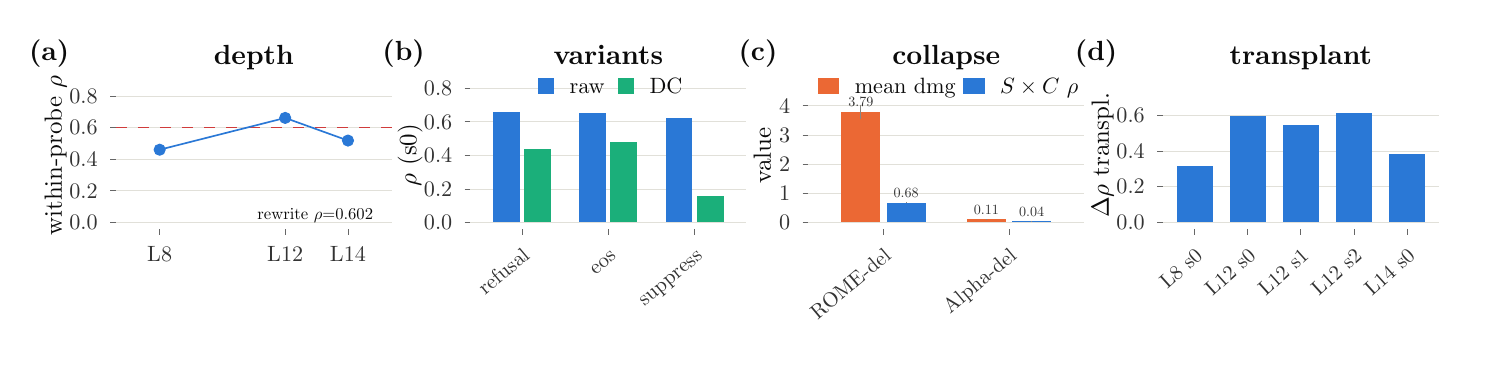
\begin{tikzpicture}[x=1pt,y=1pt]
\definecolor{fillColor}{RGB}{255,255,255}
\path[use as bounding box,fill=fillColor,fill opacity=0.00] (0,0) rectangle (517.45,112.02);
\begin{scope}
\path[clip] (  0.00,  0.00) rectangle (517.45,112.02);
\definecolor{drawColor}{RGB}{255,255,255}
\definecolor{fillColor}{RGB}{255,255,255}

\path[draw=drawColor,line width= 0.6pt,line join=round,line cap=round,fill=fillColor] (  0.00,  0.00) rectangle (517.45,112.02);
\end{scope}
\begin{scope}
\path[clip] (  5.50,  5.50) rectangle (133.61,106.52);
\definecolor{fillColor}{RGB}{255,255,255}

\path[fill=fillColor] (  5.50,  5.50) rectangle (133.61,106.52);
\end{scope}
\begin{scope}
\path[clip] (133.61,  5.50) rectangle (261.73,106.52);
\definecolor{fillColor}{RGB}{255,255,255}

\path[fill=fillColor] (133.61,  5.50) rectangle (261.73,106.52);
\end{scope}
\begin{scope}
\path[clip] (261.73,  5.50) rectangle (383.84,106.52);
\definecolor{fillColor}{RGB}{255,255,255}

\path[fill=fillColor] (261.73,  5.50) rectangle (383.84,106.52);
\end{scope}
\begin{scope}
\path[clip] (383.84,  5.50) rectangle (511.95,106.52);
\definecolor{fillColor}{RGB}{255,255,255}

\path[fill=fillColor] (383.84,  5.50) rectangle (511.95,106.52);
\end{scope}
\begin{scope}
\path[clip] ( 31.81, 39.22) rectangle (131.61, 92.52);
\definecolor{drawColor}{RGB}{225,224,217}

\path[draw=drawColor,line width= 0.3pt,line join=round] ( 31.81, 41.64) --
	(131.61, 41.64);

\path[draw=drawColor,line width= 0.3pt,line join=round] ( 31.81, 53.04) --
	(131.61, 53.04);

\path[draw=drawColor,line width= 0.3pt,line join=round] ( 31.81, 64.44) --
	(131.61, 64.44);

\path[draw=drawColor,line width= 0.3pt,line join=round] ( 31.81, 75.85) --
	(131.61, 75.85);

\path[draw=drawColor,line width= 0.3pt,line join=round] ( 31.81, 87.25) --
	(131.61, 87.25);
\definecolor{drawColor}{RGB}{208,59,59}

\path[draw=drawColor,line width= 0.5pt,dash pattern=on 4pt off 4pt ,line join=round] ( 31.81, 75.95) -- (131.61, 75.95);
\definecolor{drawColor}{RGB}{11,11,11}

\node[text=drawColor,anchor=base east,inner sep=0pt, outer sep=0pt, scale=  0.60] at (124.81, 42.54) {rewrite $\rho{=}0.602$};
\definecolor{drawColor}{RGB}{137,135,129}

\path[draw=drawColor,line width= 0.4pt,line join=round] ( 47.69, 68.89) --
	( 47.69, 68.89);

\path[draw=drawColor,line width= 0.4pt,line join=round] ( 47.69, 68.89) --
	( 47.69, 66.95);

\path[draw=drawColor,line width= 0.4pt,line join=round] ( 47.69, 66.95) --
	( 47.69, 66.95);

\path[draw=drawColor,line width= 0.4pt,line join=round] ( 93.05, 80.47) --
	( 93.05, 80.47);

\path[draw=drawColor,line width= 0.4pt,line join=round] ( 93.05, 80.47) --
	( 93.05, 78.36);

\path[draw=drawColor,line width= 0.4pt,line join=round] ( 93.05, 78.36) --
	( 93.05, 78.36);

\path[draw=drawColor,line width= 0.4pt,line join=round] (115.74, 72.24) --
	(115.74, 72.24);

\path[draw=drawColor,line width= 0.4pt,line join=round] (115.74, 72.24) --
	(115.74, 70.23);

\path[draw=drawColor,line width= 0.4pt,line join=round] (115.74, 70.23) --
	(115.74, 70.23);
\definecolor{drawColor}{RGB}{42,120,214}

\path[draw=drawColor,line width= 0.6pt,line join=round] ( 47.69, 67.92) --
	( 93.05, 79.41) --
	(115.74, 71.23);
\definecolor{fillColor}{RGB}{42,120,214}

\path[draw=drawColor,line width= 0.3pt,line join=round,line cap=round,fill=fillColor] ( 47.69, 67.92) circle (  2.04);

\path[draw=drawColor,line width= 0.3pt,line join=round,line cap=round,fill=fillColor] ( 93.05, 79.41) circle (  2.04);

\path[draw=drawColor,line width= 0.3pt,line join=round,line cap=round,fill=fillColor] (115.74, 71.23) circle (  2.04);
\end{scope}
\begin{scope}
\path[clip] (  0.00,  0.00) rectangle (517.45,112.02);
\definecolor{drawColor}{gray}{0.20}

\node[text=drawColor,anchor=base east,inner sep=0pt, outer sep=0pt, scale=  0.80] at ( 25.31, 39.03) {0.0};

\node[text=drawColor,anchor=base east,inner sep=0pt, outer sep=0pt, scale=  0.80] at ( 25.31, 50.44) {0.2};

\node[text=drawColor,anchor=base east,inner sep=0pt, outer sep=0pt, scale=  0.80] at ( 25.31, 61.84) {0.4};

\node[text=drawColor,anchor=base east,inner sep=0pt, outer sep=0pt, scale=  0.80] at ( 25.31, 73.24) {0.6};

\node[text=drawColor,anchor=base east,inner sep=0pt, outer sep=0pt, scale=  0.80] at ( 25.31, 84.65) {0.8};
\end{scope}
\begin{scope}
\path[clip] (  0.00,  0.00) rectangle (517.45,112.02);
\definecolor{drawColor}{gray}{0.40}

\path[draw=drawColor,line width= 0.3pt,line join=round] ( 29.81, 41.64) --
	( 31.81, 41.64);

\path[draw=drawColor,line width= 0.3pt,line join=round] ( 29.81, 53.04) --
	( 31.81, 53.04);

\path[draw=drawColor,line width= 0.3pt,line join=round] ( 29.81, 64.44) --
	( 31.81, 64.44);

\path[draw=drawColor,line width= 0.3pt,line join=round] ( 29.81, 75.85) --
	( 31.81, 75.85);

\path[draw=drawColor,line width= 0.3pt,line join=round] ( 29.81, 87.25) --
	( 31.81, 87.25);
\end{scope}
\begin{scope}
\path[clip] (  0.00,  0.00) rectangle (517.45,112.02);
\definecolor{drawColor}{gray}{0.40}

\path[draw=drawColor,line width= 0.3pt,line join=round] ( 47.69, 37.22) --
	( 47.69, 39.22);

\path[draw=drawColor,line width= 0.3pt,line join=round] ( 93.05, 37.22) --
	( 93.05, 39.22);

\path[draw=drawColor,line width= 0.3pt,line join=round] (115.74, 37.22) --
	(115.74, 39.22);
\end{scope}
\begin{scope}
\path[clip] (  0.00,  0.00) rectangle (517.45,112.02);
\definecolor{drawColor}{gray}{0.20}

\node[text=drawColor,anchor=base,inner sep=0pt, outer sep=0pt, scale=  0.80] at ( 47.69, 27.51) {L8};

\node[text=drawColor,anchor=base,inner sep=0pt, outer sep=0pt, scale=  0.80] at ( 93.05, 27.51) {L12};

\node[text=drawColor,anchor=base,inner sep=0pt, outer sep=0pt, scale=  0.80] at (115.74, 27.51) {L14};
\end{scope}
\begin{scope}
\path[clip] (  0.00,  0.00) rectangle (517.45,112.02);
\definecolor{drawColor}{RGB}{11,11,11}

\node[text=drawColor,rotate= 90.00,anchor=base,inner sep=0pt, outer sep=0pt, scale=  0.90] at ( 12.36, 65.87) {within-probe $\rho$};
\end{scope}
\begin{scope}
\path[clip] (  0.00,  0.00) rectangle (517.45,112.02);
\definecolor{drawColor}{RGB}{11,11,11}

\node[text=drawColor,anchor=base,inner sep=0pt, outer sep=0pt, scale=  1.00] at ( 81.71, 98.63) {\bfseries depth};
\end{scope}
\begin{scope}
\path[clip] (  0.00,  0.00) rectangle (517.45,112.02);
\definecolor{drawColor}{RGB}{11,11,11}

\node[text=drawColor,anchor=base,inner sep=0pt, outer sep=0pt, scale=  1.00] at (  7.75,100.09) {\bfseries (a)};
\end{scope}
\begin{scope}
\path[clip] (159.92, 39.22) rectangle (259.73, 92.52);
\definecolor{drawColor}{RGB}{225,224,217}

\path[draw=drawColor,line width= 0.3pt,line join=round] (159.92, 41.64) --
	(259.73, 41.64);

\path[draw=drawColor,line width= 0.3pt,line join=round] (159.92, 53.75) --
	(259.73, 53.75);

\path[draw=drawColor,line width= 0.3pt,line join=round] (159.92, 65.87) --
	(259.73, 65.87);

\path[draw=drawColor,line width= 0.3pt,line join=round] (159.92, 77.99) --
	(259.73, 77.99);

\path[draw=drawColor,line width= 0.3pt,line join=round] (159.92, 90.10) --
	(259.73, 90.10);
\definecolor{fillColor}{RGB}{42,120,214}

\path[fill=fillColor] (168.19, 41.64) rectangle (177.85, 81.44);
\definecolor{fillColor}{RGB}{27,175,122}

\path[fill=fillColor] (179.41, 41.64) rectangle (189.08, 68.12);
\definecolor{fillColor}{RGB}{42,120,214}

\path[fill=fillColor] (199.38, 41.64) rectangle (209.04, 81.20);
\definecolor{fillColor}{RGB}{27,175,122}

\path[fill=fillColor] (210.60, 41.64) rectangle (220.27, 70.86);
\definecolor{fillColor}{RGB}{42,120,214}

\path[fill=fillColor] (230.56, 41.64) rectangle (240.23, 79.28);
\definecolor{fillColor}{RGB}{27,175,122}

\path[fill=fillColor] (241.79, 41.64) rectangle (251.46, 51.25);
\end{scope}
\begin{scope}
\path[clip] (  0.00,  0.00) rectangle (517.45,112.02);
\definecolor{drawColor}{gray}{0.20}

\node[text=drawColor,anchor=base east,inner sep=0pt, outer sep=0pt, scale=  0.80] at (153.42, 39.03) {0.0};

\node[text=drawColor,anchor=base east,inner sep=0pt, outer sep=0pt, scale=  0.80] at (153.42, 51.15) {0.2};

\node[text=drawColor,anchor=base east,inner sep=0pt, outer sep=0pt, scale=  0.80] at (153.42, 63.27) {0.4};

\node[text=drawColor,anchor=base east,inner sep=0pt, outer sep=0pt, scale=  0.80] at (153.42, 75.38) {0.6};

\node[text=drawColor,anchor=base east,inner sep=0pt, outer sep=0pt, scale=  0.80] at (153.42, 87.50) {0.8};
\end{scope}
\begin{scope}
\path[clip] (  0.00,  0.00) rectangle (517.45,112.02);
\definecolor{drawColor}{gray}{0.40}

\path[draw=drawColor,line width= 0.3pt,line join=round] (157.92, 41.64) --
	(159.92, 41.64);

\path[draw=drawColor,line width= 0.3pt,line join=round] (157.92, 53.75) --
	(159.92, 53.75);

\path[draw=drawColor,line width= 0.3pt,line join=round] (157.92, 65.87) --
	(159.92, 65.87);

\path[draw=drawColor,line width= 0.3pt,line join=round] (157.92, 77.99) --
	(159.92, 77.99);

\path[draw=drawColor,line width= 0.3pt,line join=round] (157.92, 90.10) --
	(159.92, 90.10);
\end{scope}
\begin{scope}
\path[clip] (  0.00,  0.00) rectangle (517.45,112.02);
\definecolor{drawColor}{gray}{0.40}

\path[draw=drawColor,line width= 0.3pt,line join=round] (178.63, 37.22) --
	(178.63, 39.22);

\path[draw=drawColor,line width= 0.3pt,line join=round] (209.82, 37.22) --
	(209.82, 39.22);

\path[draw=drawColor,line width= 0.3pt,line join=round] (241.01, 37.22) --
	(241.01, 39.22);
\end{scope}
\begin{scope}
\path[clip] (  0.00,  0.00) rectangle (517.45,112.02);
\definecolor{drawColor}{gray}{0.20}

\node[text=drawColor,rotate= 40.00,anchor=base east,inner sep=0pt, outer sep=0pt, scale=  0.75] at (181.77, 28.97) {refusal};

\node[text=drawColor,rotate= 40.00,anchor=base east,inner sep=0pt, outer sep=0pt, scale=  0.75] at (212.96, 28.97) {eos};

\node[text=drawColor,rotate= 40.00,anchor=base east,inner sep=0pt, outer sep=0pt, scale=  0.75] at (244.15, 28.97) {suppress};
\end{scope}
\begin{scope}
\path[clip] (  0.00,  0.00) rectangle (517.45,112.02);
\definecolor{drawColor}{RGB}{11,11,11}

\node[text=drawColor,rotate= 90.00,anchor=base,inner sep=0pt, outer sep=0pt, scale=  0.90] at (140.47, 65.87) {$\rho$ (s0)};
\end{scope}
\begin{scope}
\path[clip] (  0.00,  0.00) rectangle (517.45,112.02);
\definecolor{fillColor}{RGB}{42,120,214}

\path[fill=fillColor] (184.48, 88.17) rectangle (190.18, 93.82);
\end{scope}
\begin{scope}
\path[clip] (  0.00,  0.00) rectangle (517.45,112.02);
\definecolor{fillColor}{RGB}{27,175,122}

\path[fill=fillColor] (213.35, 88.17) rectangle (219.06, 93.82);
\end{scope}
\begin{scope}
\path[clip] (  0.00,  0.00) rectangle (517.45,112.02);
\definecolor{drawColor}{RGB}{11,11,11}

\node[text=drawColor,anchor=base west,inner sep=0pt, outer sep=0pt, scale=  0.80] at (195.83, 88.39) {raw};
\end{scope}
\begin{scope}
\path[clip] (  0.00,  0.00) rectangle (517.45,112.02);
\definecolor{drawColor}{RGB}{11,11,11}

\node[text=drawColor,anchor=base west,inner sep=0pt, outer sep=0pt, scale=  0.80] at (224.70, 88.39) {DC};
\end{scope}
\begin{scope}
\path[clip] (  0.00,  0.00) rectangle (517.45,112.02);
\definecolor{drawColor}{RGB}{11,11,11}

\node[text=drawColor,anchor=base,inner sep=0pt, outer sep=0pt, scale=  1.00] at (209.82, 98.63) {\bfseries variants};
\end{scope}
\begin{scope}
\path[clip] (  0.00,  0.00) rectangle (517.45,112.02);
\definecolor{drawColor}{RGB}{11,11,11}

\node[text=drawColor,anchor=base,inner sep=0pt, outer sep=0pt, scale=  1.00] at (135.86,100.09) {\bfseries (b)};
\end{scope}
\begin{scope}
\path[clip] (282.03, 39.22) rectangle (381.84, 92.52);
\definecolor{drawColor}{RGB}{225,224,217}

\path[draw=drawColor,line width= 0.3pt,line join=round] (282.03, 41.64) --
	(381.84, 41.64);

\path[draw=drawColor,line width= 0.3pt,line join=round] (282.03, 52.17) --
	(381.84, 52.17);

\path[draw=drawColor,line width= 0.3pt,line join=round] (282.03, 62.71) --
	(381.84, 62.71);

\path[draw=drawColor,line width= 0.3pt,line join=round] (282.03, 73.24) --
	(381.84, 73.24);

\path[draw=drawColor,line width= 0.3pt,line join=round] (282.03, 83.78) --
	(381.84, 83.78);
\definecolor{fillColor}{RGB}{235,104,52}

\path[fill=fillColor] (294.06, 41.64) rectangle (308.12, 81.55);

\path[fill=fillColor] (339.42, 41.64) rectangle (353.49, 42.75);
\definecolor{fillColor}{RGB}{42,120,214}

\path[fill=fillColor] (310.39, 41.64) rectangle (324.45, 48.78);

\path[fill=fillColor] (355.75, 41.64) rectangle (369.82, 42.02);
\definecolor{drawColor}{RGB}{137,135,129}

\path[draw=drawColor,line width= 0.4pt,line join=round] (301.09, 84.24) --
	(301.09, 84.24);

\path[draw=drawColor,line width= 0.4pt,line join=round] (301.09, 84.24) --
	(301.09, 78.87);

\path[draw=drawColor,line width= 0.4pt,line join=round] (301.09, 78.87) --
	(301.09, 78.87);

\path[draw=drawColor,line width= 0.4pt,line join=round] (346.45, 42.79) --
	(346.45, 42.79);

\path[draw=drawColor,line width= 0.4pt,line join=round] (346.45, 42.79) --
	(346.45, 42.71);

\path[draw=drawColor,line width= 0.4pt,line join=round] (346.45, 42.71) --
	(346.45, 42.71);

\path[draw=drawColor,line width= 0.4pt,line join=round] (317.42, 48.95) --
	(317.42, 48.95);

\path[draw=drawColor,line width= 0.4pt,line join=round] (317.42, 48.95) --
	(317.42, 48.61);

\path[draw=drawColor,line width= 0.4pt,line join=round] (317.42, 48.61) --
	(317.42, 48.61);

\path[draw=drawColor,line width= 0.4pt,line join=round] (362.79, 42.17) --
	(362.79, 42.17);

\path[draw=drawColor,line width= 0.4pt,line join=round] (362.79, 42.17) --
	(362.79, 41.87);

\path[draw=drawColor,line width= 0.4pt,line join=round] (362.79, 41.87) --
	(362.79, 41.87);
\definecolor{drawColor}{gray}{0.20}

\node[text=drawColor,anchor=base,inner sep=0pt, outer sep=0pt, scale=  0.51] at (301.09, 83.39) {3.79};

\node[text=drawColor,anchor=base,inner sep=0pt, outer sep=0pt, scale=  0.51] at (346.45, 44.58) {0.11};

\node[text=drawColor,anchor=base,inner sep=0pt, outer sep=0pt, scale=  0.51] at (317.42, 50.61) {0.68};

\node[text=drawColor,anchor=base,inner sep=0pt, outer sep=0pt, scale=  0.51] at (362.79, 43.85) {0.04};
\end{scope}
\begin{scope}
\path[clip] (  0.00,  0.00) rectangle (517.45,112.02);
\definecolor{drawColor}{gray}{0.20}

\node[text=drawColor,anchor=base east,inner sep=0pt, outer sep=0pt, scale=  0.80] at (275.53, 39.03) {0};

\node[text=drawColor,anchor=base east,inner sep=0pt, outer sep=0pt, scale=  0.80] at (275.53, 49.57) {1};

\node[text=drawColor,anchor=base east,inner sep=0pt, outer sep=0pt, scale=  0.80] at (275.53, 60.10) {2};

\node[text=drawColor,anchor=base east,inner sep=0pt, outer sep=0pt, scale=  0.80] at (275.53, 70.64) {3};

\node[text=drawColor,anchor=base east,inner sep=0pt, outer sep=0pt, scale=  0.80] at (275.53, 81.18) {4};
\end{scope}
\begin{scope}
\path[clip] (  0.00,  0.00) rectangle (517.45,112.02);
\definecolor{drawColor}{gray}{0.40}

\path[draw=drawColor,line width= 0.3pt,line join=round] (280.03, 41.64) --
	(282.03, 41.64);

\path[draw=drawColor,line width= 0.3pt,line join=round] (280.03, 52.17) --
	(282.03, 52.17);

\path[draw=drawColor,line width= 0.3pt,line join=round] (280.03, 62.71) --
	(282.03, 62.71);

\path[draw=drawColor,line width= 0.3pt,line join=round] (280.03, 73.24) --
	(282.03, 73.24);

\path[draw=drawColor,line width= 0.3pt,line join=round] (280.03, 83.78) --
	(282.03, 83.78);
\end{scope}
\begin{scope}
\path[clip] (  0.00,  0.00) rectangle (517.45,112.02);
\definecolor{drawColor}{gray}{0.40}

\path[draw=drawColor,line width= 0.3pt,line join=round] (309.25, 37.22) --
	(309.25, 39.22);

\path[draw=drawColor,line width= 0.3pt,line join=round] (354.62, 37.22) --
	(354.62, 39.22);
\end{scope}
\begin{scope}
\path[clip] (  0.00,  0.00) rectangle (517.45,112.02);
\definecolor{drawColor}{gray}{0.20}

\node[text=drawColor,rotate= 40.00,anchor=base east,inner sep=0pt, outer sep=0pt, scale=  0.75] at (312.39, 28.97) {ROME-del};

\node[text=drawColor,rotate= 40.00,anchor=base east,inner sep=0pt, outer sep=0pt, scale=  0.75] at (357.76, 28.97) {Alpha-del};
\end{scope}
\begin{scope}
\path[clip] (  0.00,  0.00) rectangle (517.45,112.02);
\definecolor{drawColor}{RGB}{11,11,11}

\node[text=drawColor,rotate= 90.00,anchor=base,inner sep=0pt, outer sep=0pt, scale=  0.90] at (268.59, 65.87) {value};
\end{scope}
\begin{scope}
\path[clip] (  0.00,  0.00) rectangle (517.45,112.02);
\definecolor{fillColor}{RGB}{235,104,52}

\path[fill=fillColor] (285.52, 88.17) rectangle (293.23, 93.82);
\end{scope}
\begin{scope}
\path[clip] (  0.00,  0.00) rectangle (517.45,112.02);
\definecolor{fillColor}{RGB}{42,120,214}

\path[fill=fillColor] (338.07, 88.17) rectangle (345.78, 93.82);
\end{scope}
\begin{scope}
\path[clip] (  0.00,  0.00) rectangle (517.45,112.02);
\definecolor{drawColor}{RGB}{11,11,11}

\node[text=drawColor,anchor=base west,inner sep=0pt, outer sep=0pt, scale=  0.80] at (298.88, 88.39) {mean dmg};
\end{scope}
\begin{scope}
\path[clip] (  0.00,  0.00) rectangle (517.45,112.02);
\definecolor{drawColor}{RGB}{11,11,11}

\node[text=drawColor,anchor=base west,inner sep=0pt, outer sep=0pt, scale=  0.80] at (351.43, 88.39) {$S\times C$ $\rho$};
\end{scope}
\begin{scope}
\path[clip] (  0.00,  0.00) rectangle (517.45,112.02);
\definecolor{drawColor}{RGB}{11,11,11}

\node[text=drawColor,anchor=base,inner sep=0pt, outer sep=0pt, scale=  1.00] at (331.94, 98.63) {\bfseries collapse};
\end{scope}
\begin{scope}
\path[clip] (  0.00,  0.00) rectangle (517.45,112.02);
\definecolor{drawColor}{RGB}{11,11,11}

\node[text=drawColor,anchor=base,inner sep=0pt, outer sep=0pt, scale=  1.00] at (263.92,100.09) {\bfseries (c)};
\end{scope}
\begin{scope}
\path[clip] (410.15, 39.22) rectangle (509.95, 92.52);
\definecolor{drawColor}{RGB}{225,224,217}

\path[draw=drawColor,line width= 0.3pt,line join=round] (410.15, 41.64) --
	(509.95, 41.64);

\path[draw=drawColor,line width= 0.3pt,line join=round] (410.15, 54.56) --
	(509.95, 54.56);

\path[draw=drawColor,line width= 0.3pt,line join=round] (410.15, 67.48) --
	(509.95, 67.48);

\path[draw=drawColor,line width= 0.3pt,line join=round] (410.15, 80.41) --
	(509.95, 80.41);
\definecolor{fillColor}{RGB}{42,120,214}

\path[fill=fillColor] (415.14, 41.64) rectangle (428.19, 61.93);

\path[fill=fillColor] (434.33, 41.64) rectangle (447.38, 79.99);

\path[fill=fillColor] (453.52, 41.64) rectangle (466.58, 76.91);

\path[fill=fillColor] (472.72, 41.64) rectangle (485.77, 81.21);

\path[fill=fillColor] (491.91, 41.64) rectangle (504.96, 66.44);
\end{scope}
\begin{scope}
\path[clip] (  0.00,  0.00) rectangle (517.45,112.02);
\definecolor{drawColor}{gray}{0.20}

\node[text=drawColor,anchor=base east,inner sep=0pt, outer sep=0pt, scale=  0.80] at (403.65, 39.03) {0.0};

\node[text=drawColor,anchor=base east,inner sep=0pt, outer sep=0pt, scale=  0.80] at (403.65, 51.96) {0.2};

\node[text=drawColor,anchor=base east,inner sep=0pt, outer sep=0pt, scale=  0.80] at (403.65, 64.88) {0.4};

\node[text=drawColor,anchor=base east,inner sep=0pt, outer sep=0pt, scale=  0.80] at (403.65, 77.80) {0.6};
\end{scope}
\begin{scope}
\path[clip] (  0.00,  0.00) rectangle (517.45,112.02);
\definecolor{drawColor}{gray}{0.40}

\path[draw=drawColor,line width= 0.3pt,line join=round] (408.15, 41.64) --
	(410.15, 41.64);

\path[draw=drawColor,line width= 0.3pt,line join=round] (408.15, 54.56) --
	(410.15, 54.56);

\path[draw=drawColor,line width= 0.3pt,line join=round] (408.15, 67.48) --
	(410.15, 67.48);

\path[draw=drawColor,line width= 0.3pt,line join=round] (408.15, 80.41) --
	(410.15, 80.41);
\end{scope}
\begin{scope}
\path[clip] (  0.00,  0.00) rectangle (517.45,112.02);
\definecolor{drawColor}{gray}{0.40}

\path[draw=drawColor,line width= 0.3pt,line join=round] (421.66, 37.22) --
	(421.66, 39.22);

\path[draw=drawColor,line width= 0.3pt,line join=round] (440.86, 37.22) --
	(440.86, 39.22);

\path[draw=drawColor,line width= 0.3pt,line join=round] (460.05, 37.22) --
	(460.05, 39.22);

\path[draw=drawColor,line width= 0.3pt,line join=round] (479.24, 37.22) --
	(479.24, 39.22);

\path[draw=drawColor,line width= 0.3pt,line join=round] (498.44, 37.22) --
	(498.44, 39.22);
\end{scope}
\begin{scope}
\path[clip] (  0.00,  0.00) rectangle (517.45,112.02);
\definecolor{drawColor}{gray}{0.20}

\node[text=drawColor,rotate= 42.00,anchor=base east,inner sep=0pt, outer sep=0pt, scale=  0.75] at (424.93, 29.09) {L8 s0};

\node[text=drawColor,rotate= 42.00,anchor=base east,inner sep=0pt, outer sep=0pt, scale=  0.75] at (444.12, 29.09) {L12 s0};

\node[text=drawColor,rotate= 42.00,anchor=base east,inner sep=0pt, outer sep=0pt, scale=  0.75] at (463.32, 29.09) {L12 s1};

\node[text=drawColor,rotate= 42.00,anchor=base east,inner sep=0pt, outer sep=0pt, scale=  0.75] at (482.51, 29.09) {L12 s2};

\node[text=drawColor,rotate= 42.00,anchor=base east,inner sep=0pt, outer sep=0pt, scale=  0.75] at (501.70, 29.09) {L14 s0};
\end{scope}
\begin{scope}
\path[clip] (  0.00,  0.00) rectangle (517.45,112.02);
\definecolor{drawColor}{RGB}{11,11,11}

\node[text=drawColor,rotate= 90.00,anchor=base,inner sep=0pt, outer sep=0pt, scale=  0.90] at (390.70, 65.87) {$\Delta\rho$ transpl.};
\end{scope}
\begin{scope}
\path[clip] (  0.00,  0.00) rectangle (517.45,112.02);
\definecolor{drawColor}{RGB}{11,11,11}

\node[text=drawColor,anchor=base,inner sep=0pt, outer sep=0pt, scale=  1.00] at (460.05, 98.63) {\bfseries transplant};
\end{scope}
\begin{scope}
\path[clip] (  0.00,  0.00) rectangle (517.45,112.02);
\definecolor{drawColor}{RGB}{11,11,11}

\node[text=drawColor,anchor=base,inner sep=0pt, outer sep=0pt, scale=  1.00] at (386.09,100.09) {\bfseries (d)};
\end{scope}
\end{tikzpicture}
